\section{Piezos und Ultraschall}

\subsection{Grundlagen}
Piezokeramische Bauelemente wandeln mechanische Signale wie Kraft, Druck, Dehnung oder
Beschleunigung in eine elektrische Spannung um oder umgekehrt. Die typischen Resonanzfrequenzen liegen dabei zwischen 40 kHz und 10 MHz. Der piezoelektrische Effekt tritt sowohl in \textbf{einkristallinen Materialien} als auch
in \textbf{polykristallinen ferroelektrischen Keramiken} auf.
\begin{compactitem}
    \item Direkter piezoelektrischer Effekt: Bei Druckeinwirkung (wandelt mech. in elektr. Energie um)
    \item Indirekter piezoelektrischer Effekt: Bei Anlegen einer elektr. Spannung (wandelt elektr. in mech. Energie um)
\end{compactitem}

\subsubsection{Piezoelektrische Kristalle}
\begin{compactitem}
    \item Der wichtigste piezoelektrische Kristall ist die vom Quarz gebildete bis zu 573 ${^\circ}$ C stabile trigonale Kristallstruktur $\alpha$-Quarz. Die wichtigste Anwendung sind Schwingquarze.
    \item Lithiumniobat hat gegenüber Quarz höhere piezoelektrische Konstanten und wird für piezoelektrische Filter und SAW-Bauelemente (engl.: surface acoustic wave, Akustische Oberflächenwelle) verwendet.
\end{compactitem}

\subsubsection{Piezoelektrische Keramik}
Industriell hergestellte Piezoelemente sind zumeist Keramiken. Gegenüber piezoelektrischen Kristallen haben piezoelektrische Keramiken den Vorteil wesentlich höherer piezoelektrischer Koeffizienten. 
\begin{compactitem}
    \item  Bestehen aus synthetischen, anorganischen, ferroelektrischen und polykristallinen Keramikwerkstoffen
    \item Typische Basismaterialien sind modifizierte Blei-Zirkonat-Titanate (PZT) und Blei-Magnesium-Niobate (PMN)
\end{compactitem}
\textbf{Blei-Zirkonat-Titanate (PZT):}
\begin{compactitem}
    \item Unterhalb der Curie-Temperatur $T_{C}$ wird die Gitterstruktur der PZT-Kristallite verzerrt und asymmetrisch. Es entstehen Dipole und die für die Piezotechnologie interessanten rhomboedrischen bzw. tetragonalen Kristallitphasen bilden sich heraus. Die Keramik weist eine spontane Polarisation auf. Oberhalb der Curie-Temperatur verliert eine Piezokeramik ihre piezoelektrischen Eigenschaften.
    \item PZT-Piezokeramik ist in vielen Variationen (spez. Dotierungen z.B. mit Ni-, Bi-, La-Ionen) verfügbar und die am häufigsten verwendete Keramik für Aktor- oder Sensoranwendungen. 
\end{compactitem}

\subsection{Elektrische Ersatzschaltung}
Das elektromechanische Verhalten eines zu Schwingungen angeregten piezoelektrischen Körpers lässt sich mit folgendem elektrischen Ersatzschaltbild darstellen:\\ 
\begin{minipage}{0.5\textwidth}
    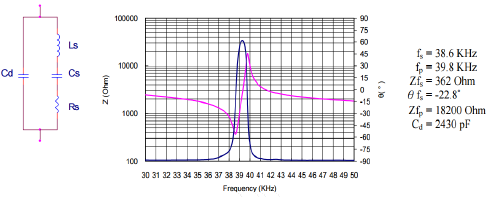
\includegraphics[width=1.0\textwidth]{images/Ersatzschaltbild_Piezo}
\end{minipage}
\hfill
\begin{minipage}{0.45\textwidth}
    \textbf{Schwingkreisbeschreibung bei Frequenzen in der nähe der mech. Eigenresonanz:}
    \begin{compactitem}
        \item $C_{0}$ $\rightarrow$  Kapazität des Dielektrikums
        \item Reihenschaltung $C_{1}$, $L_{1}$, $R_{1}$ $\rightarrow$ beschreibt die Änderung
        der mechanischen Eigenschaften wie elastische Deformation, effektive Masse (Trägheit) und mechanische Verluste durch innere Reibung\\
    \end{compactitem}
    $Z1 = s\cdot L1 + \frac{1}{s\cdot C1} + R1$ \ \ \ \ $Z2 = \frac{1}{s\cdot C0}$ \\\\ $\rightarrow$ $Zpiezo = \frac{(s\cdot L1 + \frac{1}{s\cdot C1} + R1)\cdot \frac{1}{s\cdot C0}}{s\cdot L1 + \frac{1}{s\cdot C1} + R1 + \frac{1}{s\cdot C0}} = \frac{C1\cdot L1\cdot s^2 + C1\cdot R1\cdot s + 1}{s\cdot (C0+C1)\cdot (\frac{C0\cdot C1}{C0 + C1}\cdot L1\cdot s^2 + \frac{C0\cdot C1}{C0 + C1}\cdot R1\cdot s + 1)}$
\end{minipage}

\subsection{Piezos als Schallwandler - Buzzer}
%\subsubsection{Grundlagen}
%\textbf{Lautstärke:} Bei 2kHz liegt die Frequenz bei einem Schalldruckpegel von null Dezibel, entsprechend 20 $\mu$ Pa. \ Flüstern $\rightarrow$ ca. 20dB / Konversation $\rightarrow$ ca. 60dB / Bahnunterführung $\rightarrow$ ca. 100dB\\
%\textbf{Tonhöhe:} Infraschall $\rightarrow$ 0Hz - ca. 16Hz / Hörbarer Bereich $\rightarrow$ 16 Hz - ca. 20kHz  / Ultraschall $\rightarrow$ ab ca. 16kHz

\subsubsection{Funktionsweise}
\begin{minipage}{0.5\textwidth}
    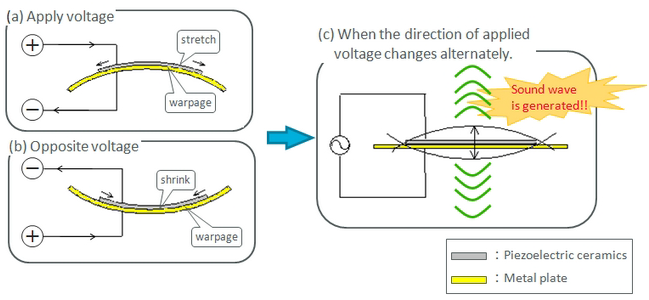
\includegraphics[width=0.8\textwidth]{images/Buzzer_Funktionsweise}
\end{minipage}
\hfill
\begin{minipage}{0.45\textwidth}
    \begin{compactitem}
        \item Metallplatte bleibt
        \item Piezo ändert Länge $\rightarrow$ biegt sich durch
        \item Höherer Schalldruck kann durch Gehäuse erzielt werden
    \end{compactitem}
\end{minipage}
\subsubsection{Funktion des Gehäuses}
 Je nach Bauform beeinflusst das Gehäuse die Schalldruckcharakteristik.
 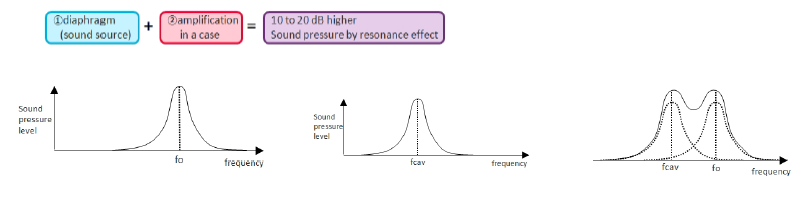
\includegraphics[width=0.8\textwidth]{images/FunktionDesGehaeuses}
\subsubsection{Oszillation}
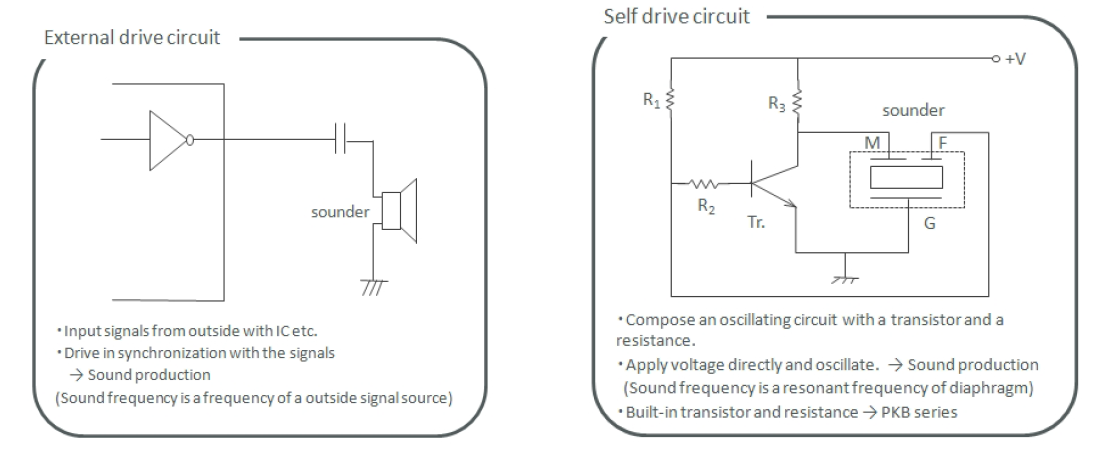
\includegraphics[width=0.6\textwidth]{images/OszillationBuzzer}

\subsection{Piezos als Schallwandler in
Ultraschall-Anwendungen für
Messtechnik - Transducer}
\subsubsection{Messverfahren}
Ultraschall-Abstands-Messung  \ \ \ \ \ \ Ultraschall-Distanz-Messung\\
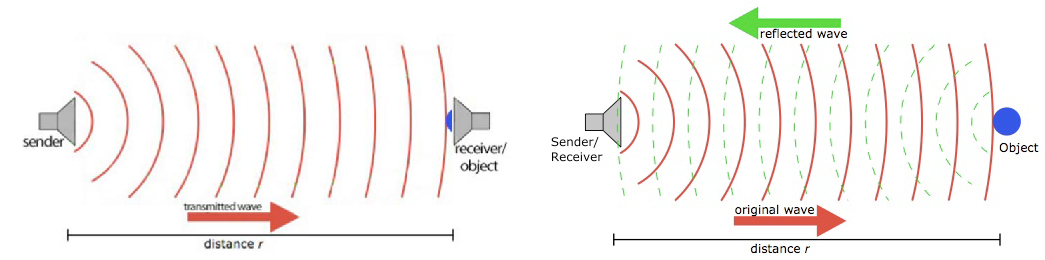
\includegraphics[width=0.6\textwidth]{images/Messverfahren}
\subsubsection{Schallausbreitung}
Energie verteilt sich mit der Zeit auf grössere Fläche. Schalldruck $\sim$ 1/Distanz\\ Bsp: Doppelte Distanz $\rightarrow$ Schall-Leistung verteilt sich auf doppelte Fläche $\rightarrow$ halber Schalldruck
\subsubsection{Absorption}
Absorption in dB/m // Faktor 10 in Frequenz $\rightarrow$ Faktor 100 in Absorption // 1MHz: 100dB/m // 100kHz: 1dB/m

\subsection{Anwendung Durchflussmessung}
\begin{minipage}{0.3\textwidth}
    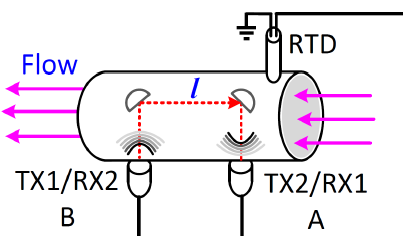
\includegraphics[width=0.8\textwidth]{images/AnwendungDurchflussmessung}   
\end{minipage}
\hfill
\begin{minipage}{0.65\textwidth}
    \begin{compactitem}
        \item Upstream TOF: $t_{BA} = \frac{l}{c-v}$
        \item Downstream TOF: $t_{AB} = \frac{l}{c+v}$
        \item Water velocity: $v = \frac{(t_{BA}-t_{AB})\cdot c^2}{2 \cdot l}$
    \end{compactitem}
\end{minipage}

\subsection{Piezos
in bildgebenden medizinischen
Ultraschall-Anwendungen}

\begin{minipage}{0.3\textwidth}
    \subsubsection{Schall-Leitung im Körper}
    Schall wird vom Gewebe reflektiert. Reflektierendes Signal wird gemessen.\\
    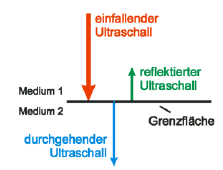
\includegraphics[width=1.0\textwidth]{images/SchallLeitung}\\\\
\end{minipage}
\hfill
\begin{minipage}{0.2\textwidth}
    \subsubsection{Brechung}
    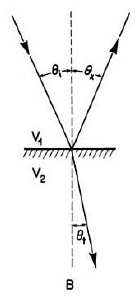
\includegraphics[width=0.4\textwidth]{images/Brechung}\\
    $\frac{sin \theta _{i}}{sin \theta _{t}} = \frac{v1}{v2}$\\\\\\\\\\\\
\end{minipage}
\hfill
\begin{minipage}{0.4\textwidth}
    \subsubsection{Beamforming}
    \begin{compactitem}
        \item Mit Transducer-Arrays kann Strahl ‘geformt’ werden
        \item Positionsabhängige Delays
    \end{compactitem}
    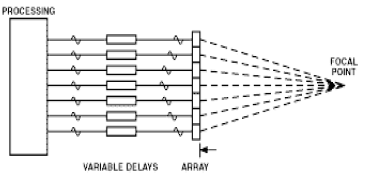
\includegraphics[width=0.6\textwidth]{images/Beamforming1}\\
    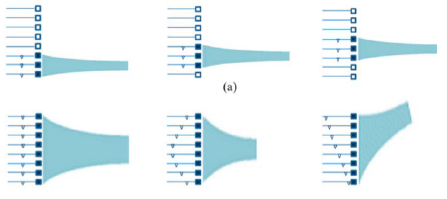
\includegraphics[width=0.8\textwidth]{images/Beamforming2}
\end{minipage}